% multi: https://texblog.org/2012/12/21/multi-column-and-multi-row-cells-in-latex-tables/

% Mit pdflatex mindestens 2mal uebersetzen und Ergebnis mit einem pdf-Viewer betrachten
%\documentclass{beamer}
% https://en.wikibooks.org/wiki/LaTeX/Colors
\documentclass[usenames,dvipsnames,handout]{beamer}
%\usepackage[latin1]{inputenc}
%\usepackage[ngerman]{babel}
\usepackage[utf8]{inputenc}
\usepackage[ngerman]{babel} 
\usepackage{color}
\usepackage{multirow,array}
%\usepackage{multirow}
\usepackage{hyperref}
\usepackage{tikz}
\usetikzlibrary{shapes.geometric, arrows}
\usetikzlibrary{fit,arrows,calc,positioning}
% http://tex.stackexchange.com/questions/33231/how-to-change-the-color-of-a-block-within-a-custom-beamer-sty-theme-file
\usepackage{color}
\definecolor{mygreen}{cmyk}{0.82,0.11,1,0.25}
\usetheme[secheader]{Boadilla}
\newenvironment{variableblock}[3]{%
  \setbeamercolor{block body}{#2}
  \setbeamercolor{block title}{#3}
  \begin{block}{#1}}{\end{block}}


\begin{document}
\author[Dr. Mariana Nold]{Dr. Mariana Nold}
% \begin{center}
\institute[Institut für Soziologie]{ Institut für Soziologie,\\ Fakultät für Sozial- und Verhaltenswissenschaften,\\ Lehrstuhl für
 empirische Sozialforschung und Sozialstrukturanalyse}
% \end{center}
 \date{}
\title [Punktschätzer und Konfidenzintervalle ]{Punktschätzer und Konfidenzintervalle }
\date{27. November 2017}
\begin{frame}
\maketitle

  \begin{figure}[ht]
 	\centering
 	      
\includegraphics[width=0.15\textwidth]{index.jpeg}
 	\end{figure}
\end{frame} 

\begin{frame}
  \frametitle{Übersicht}
  \tableofcontents
\end{frame}

\section{Themen und Ziele}




%http://www.statmethods.net/stats/power.html

\begin{frame}{Ziel der heutigen Veranstaltung \dots}
ist es die folgenden Fragen beantworten zu können:
\begin{block}{Zielfragen für heute}
\begin{enumerate}
\item{Welche Probleme treten auf, wenn man den Fehler 2. Art nicht berücksichtigt?}
\item{Wie ist die Power eines Tests definiert?}
\item{Ziel 3}
\item{Ziel 4}
\item{Ziel 5}
\item{Ziel 6}
\end{enumerate}
\end{block}
\end{frame}
\section{Stichprobenumfang und Power}

\begin{frame}{Kritik am klassischen statistischen Testen }
(vgl. LMLG S. 136 ff und 166 ff)
\begin{itemize}
\item{Statistisches Testen spielt in der Praxis der empirischen Sozialforschung einer herausragende Rolle.}\pause
\item{Tatsächlich ist sowohl das Konzept der statistischen Signifikanz als auch die Logik des statistischen
Testens überhaupt seit Jahrzehnten der Kritik ausgesetzt.}\pause
\item{Immer wieder haben renommierte Wissenschaftler gefordert, man solle statistische Signifikanztests
abschaffen. }\pause
\item{Ich möchte heute einen Kritikpunkt vorstellen und eine Möglichkeit die mit weniger Nachteilen
verbunden ist.}
\end{itemize}
\end{frame}
\begin{frame}{Die Füllmenge der Flaschen}
\begin{itemize}
\item{In der Aufgabe 6 des letzten Aufgabenblattes ging es um die Frage, ob eine Maschine die 
Mineralwasserflaschen befüllt  neu eingestellt werden muss.}\pause
\item{Die Maschine soll exakt
$500$ ml pro Flasche abfüllen. Nehmen wir an, der wahre Mittelwert der Füllmenge
ist $\mu$ und die wahre Standardabweichung $\sigma.$ Beide Parameter sind
unbekannt. Der Stichprobenumfang ist $n.$}\pause
\item{Wir wollen uns heute zunächst mit dem Fehler 2. Art beschäftigen.  Also mit dem Fehler eine unwahre 
Nullhypothese nicht zu erkennen und beizubehalten.}
\item{Es kann auch passieren, dass ein relevanter Unterschied nicht signifikant ist. Dass ist dann ein Fehler 2. Art.}
\end{itemize}
\end{frame}

\begin{frame}{Wie falsch darf die Maschine arbeiten?}
\begin{itemize}
\item{Die Toleranz wird auf $20$ ml in beide Richtungen festgelegt. Das bedeutet:
Eine Akzeptable Füllmenge liegt im Intervall $(480,520).$}\pause
\item{Die Instandsetzung der Maschine zur Neuadjustierung der Füllmenge kostet $200$ Euro.
Daher möchte die Mitarbeiterin diese nur vornehmen, wenn sie auch nötig ist.}\pause
\item{Da eine Abweichung der Füllmenge sowohl nach oben, als auch nach unten
zu Problemen führt, arbeiten mir mit der ungerichteten Null-Hypothese $H_{0}: \mu=\mu_{0}=500$}\pause
\item{Wenn also die wahre erwartete Füllmenge $490$ ml beträgt und der Test diese
Abweichung erkennt und $H_{0}$ ablehnt, dann entsteht ein Schaden von $200$ Euro.}
\end{itemize}
\end{frame}

\begin{frame}{Der Test kennt keinen Toleranzbereich}
\begin{itemize}
\item{Bitte beachten Sie: Die Nullhypothese ist schon bei der geringsten Abweichung nicht mehr
wahr. Selbst, wenn die Maschine eine erwartete Füllmenge von $503$ ml hat, ist die Nullhypothese
tatsächlich falsch.}
\item{Ein Kritikpunkt an der Praxis des statistischen Testens ist daher, dass man unterscheiden
sollte zwischen \textbf{relevanten} und \textbf{signifikanten} Unterschieden.}
\item{Es kann passieren, dass ein nicht relevanter Unterschied als signifikant nachgewiesen wird.
Das ist kein Fehler, weder ein Fehler 1. Art, noch ein Fehler 2. Art.}
\end{itemize}
\end{frame}

\begin{frame}{Power oder Stärke eines statistischen Tests}
Um zu verstehen, wie man einen statistischen Test richtig anwenden sollte, brauchen wir den 
Begriff der Power.\pause
\begin{variableblock}{Definition: Power oder Stärke eines statistischen Tests}{bg=Orchid!30,fg=black}{bg=Plum!30,fg=black}
Die Stärke eines statistischen Tests ist dessen Fähigkeit, einen in der Grundgesamtheit vorhandenen
Unterschied (oder eine andere Größe, die wir testen wollen) auch tatsächlich zu ermitteln.\\

Es gilt also: Power= 1-$\beta$ (Wahrscheinlichkeit des Fehlers 2. Art), eine hohe Power bedeutet also ein kleines
Risiko, einen Fehler 2. Art zu begehen. Eine hoher Power bedeutet aber auch ein hohes Risiko nicht relevante
Unterschiede als signifikant nachzuweisen.
\end{variableblock}
\end{frame}

\begin{frame}{Die Power und der Stichprobenumfang}
\begin{itemize}
\item{Desto höher der Stichprobenumfang ist, desto mehr empirischen Information liegt vor. Daher steigt die
Power eines Tests mit dem Stichprobenumfang.}\pause
\item{In Aufgabe 6 hatte die Mitarbeiterin 20 Flaschen getestet. Ist das ein gute Anzahl?
Wird durch diese Anzahl ein relevanter Unterschied nachweisbar?}
\item{Um diese Frage zu diskutieren, gehen Sie bitte davon aus, dass die Standardabweichung der Maschine $20$ ml beträgt.
Dieser Wert ist der Mitarbeiterin allerdings nicht bekannt.}
\end{itemize}
\end{frame}

\begin{frame}{Wie hoch ist die Power des einfachen t-Test?}
\begin{itemize}
\item{Die erwartete  Füllmenge, die wir testen wollen heißt $\mu_{0}$}\pause
\item{Die uns unbekannte wirkliche erwarte Füllmenge heißt $\mu.$}\pause
\item{Die wahre Füllmenge ist normalverteilt mit den Parameter $\mu$ und $\sigma.$}\pause
\item{Die Power dieses Test hängt von der Effektgröße $$\delta:=\frac{\mu-\mu_{0}}{\sigma}$$ ab.}\pause
\item{Für unser Beispiel gilt: $$\delta:=\frac{\mu-500}{20}$$}\pause
\item{Wie viele Flaschen sollte die Mitarbeiterin für Ihren Test verwenden?}\pause
\item{Wie viele Flaschen sollte Sie verwenden, wenn schon eine Abweichung von $10$ ml relevant wäre?}
\end{itemize}
\end{frame}

\begin{frame}{Was ist ein relevanter Unterschied?}
\begin{itemize}
\item{Die erlaubte Toleranz sind $20$ ml, also genau eine Standardabweichung.
Der Idealfall wäre, wenn der Test nur signifikant ist, wenn die Füllmenge
außerhalb des Intervalls $(480,520)$ liegt.}\pause
\item{Wenn man dieses Intervall auf die Effektgröße umrechnet, erhält man 
das Intervall $(-1,1).$}
\item{Die Grafik auf der nächsten Folie zeigt die Power des einfachen t-Test bei ungerichtete Nullhypothese $\mu=\mu_{0}=500$
für unterschiedliche Stichprobenumfänge.}
\end{itemize}
\end{frame}

\begin{frame}{Power für die Nullhypothese $\mu=\mu_{0}=500$}
  \begin{figure}[ht]
 	\centering
 	      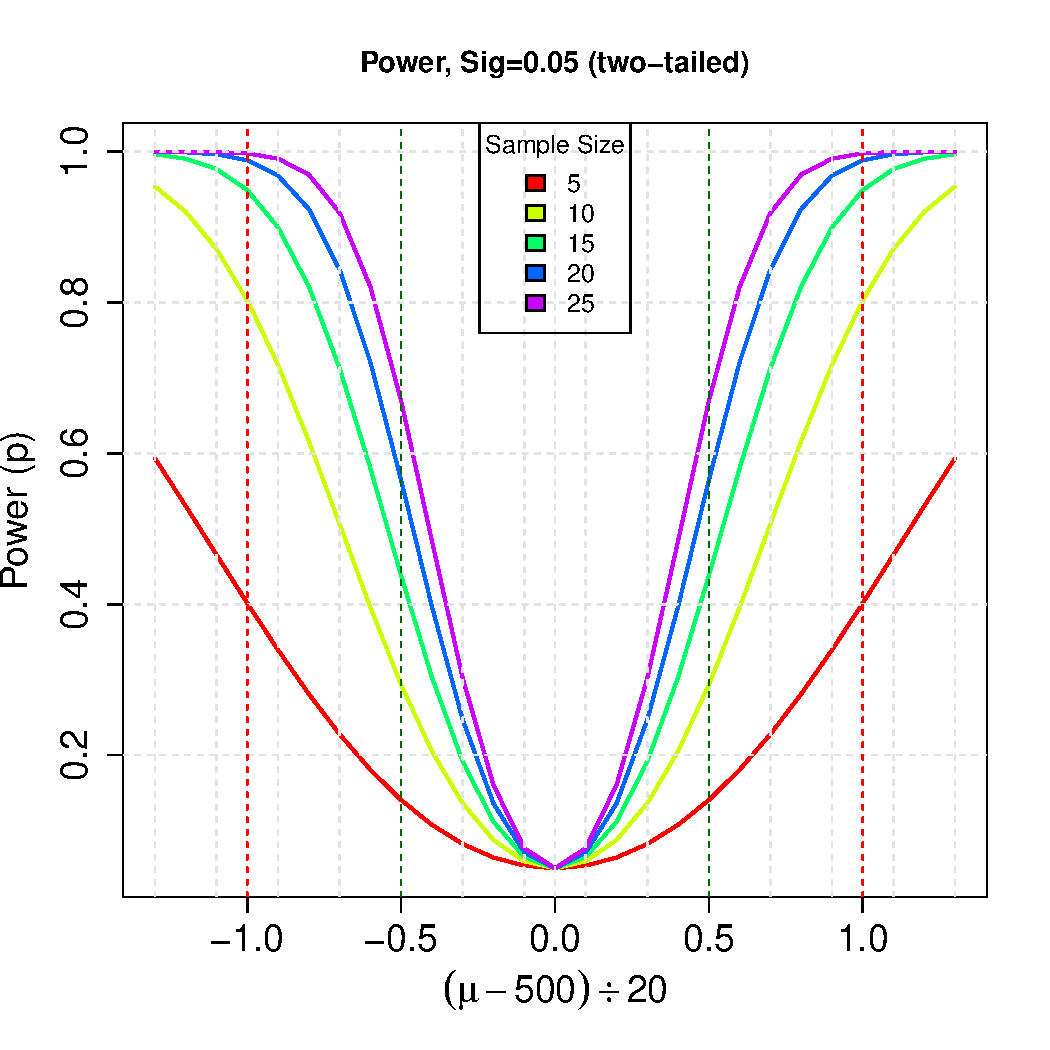
\includegraphics[width=0.65\textwidth]{power3.pdf}%{overlap3.pdf}
 	\end{figure}
\end{frame}

\begin{frame}{Ein zu großer Stichprobenumfang? }
  \begin{figure}[ht]
 	\centering
 	      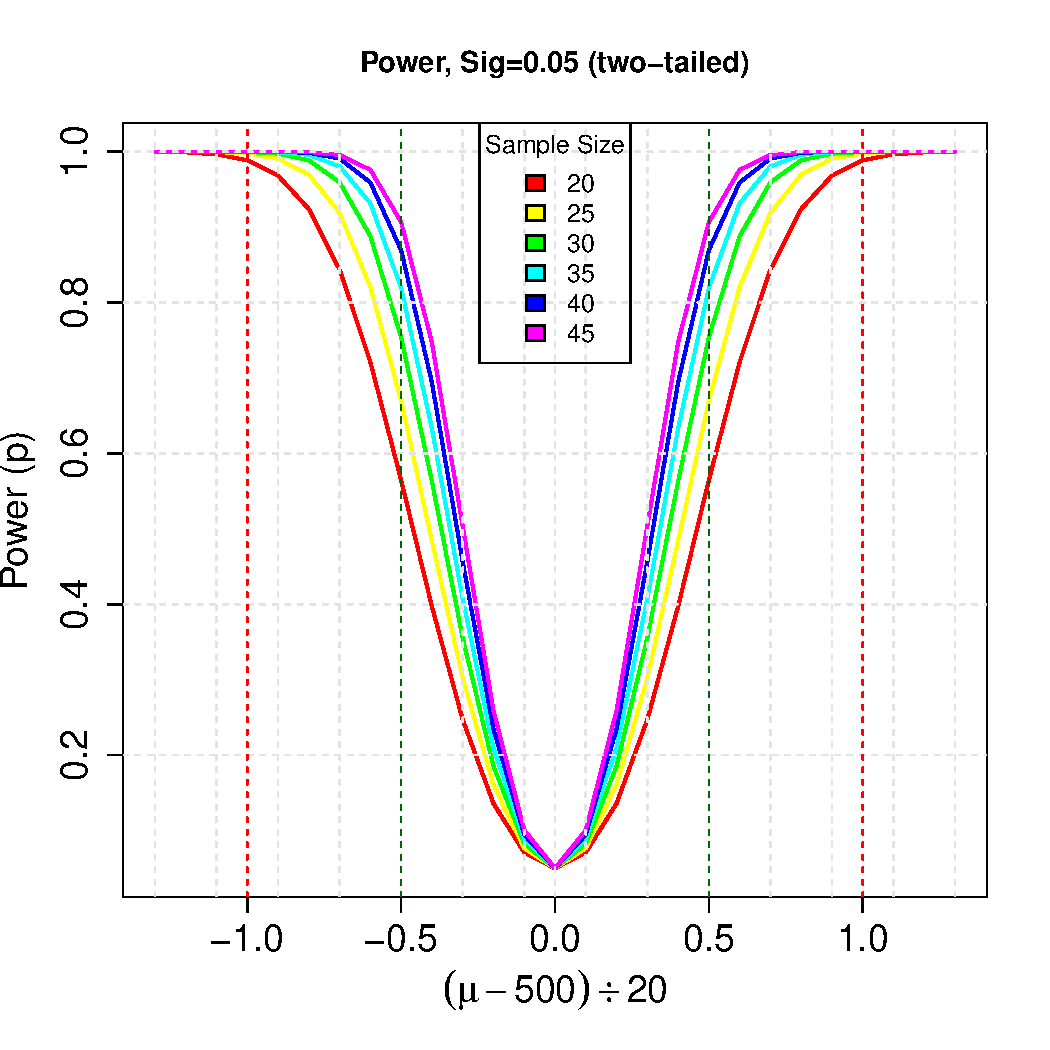
\includegraphics[width=0.65\textwidth]{power4.pdf}%{overlap3.pdf}
 	\end{figure}
\end{frame}

\begin{frame}{Statistische Tests unter Berücksichtigung der Teststärke (vgl. LMLG S. 171)}
Statistisches Testen, das unter Berücksichtigung der Ideen von Neyman und Pearson auf die Teststärke 
achtet, muss
\begin{itemize}
\item[1)]{der Nullhypothese eine eindeutige Alternativhypothese gegenüber stellen.}
\item[2)]{mit Blick auf diese Alternativhypothese (was ist relevant?) den Stichprobenumfang so
anpassen,}
\item[3)]{dass eine zufriedenstellende Teststärke erzielt wird.}
\end{itemize}\pause
Es gibt statistische Software, die die Power  für viele Tests berechnet. Es ist allerdings
die Ausnahme, dass jemand solche Software verwendet.
\end{frame}
%http://sites.nicholas.duke.edu/statsreview/ci/
%https://www.r-bloggers.com/demonstrating-confidence-intervals-with-shiny/
\begin{frame}{Statistisches Testen}
\begin{itemize}
\item{Eine vollständige Diskussion mit den Pro und Kontra-Punkten für und gegen das 
statische Test, können wir hier nicht führen.}
\item{Die bisherigen Folien geben nur einen kleinen Einblick.}
\item{Im Rest der Veranstaltung wollen wir uns mit Punktschätzern und Konfidenzintervallen
beschäftigen.}
\item{Die Auswertung der Daten mit Hilfe von Punktschätzern und Konfidenzintervallen
ist klar im Vorteil gegenüber statistischen Tests.}
\end{itemize}
\end{frame}

\begin{frame}{Übung: Lesen Mädchen besser als Jungs? }
  \begin{figure}[ht]
 	\centering
 	      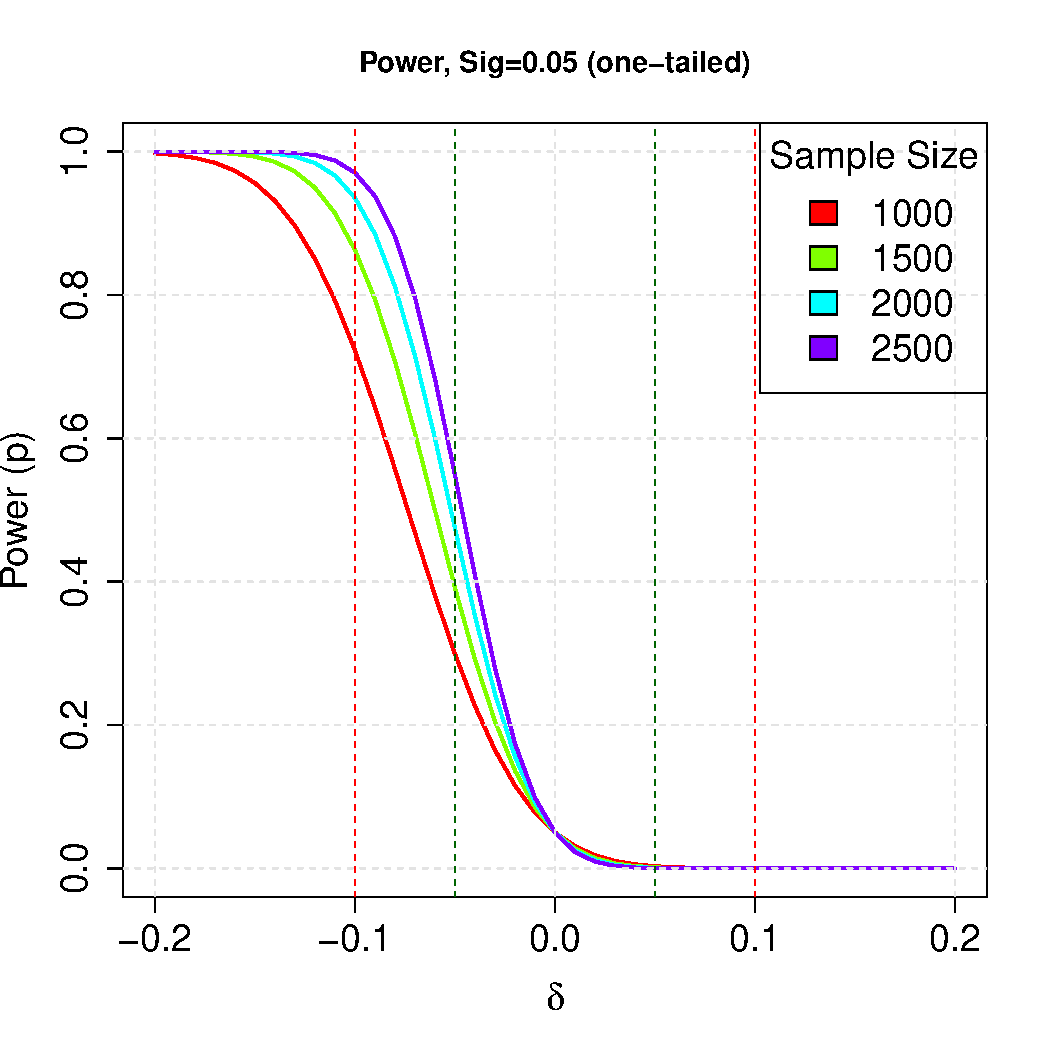
\includegraphics[width=0.65\textwidth]{powerPisa.pdf}%{overlap3.pdf}
 	\end{figure}
\end{frame}

\section{Punktschätzer für den Anteilswert}

\begin{frame}{Die diffusen Ängste der Deutschen (17.2.16)}
%http://www.faz.net/aktuell/politik/inland/allensbach-umfrage-zeigt-angst-um-innere-sicherheit-steigt-14073805/infografik-sorgen-um-die-14074061.html
  \begin{figure}[ht]
 	\centering
 	      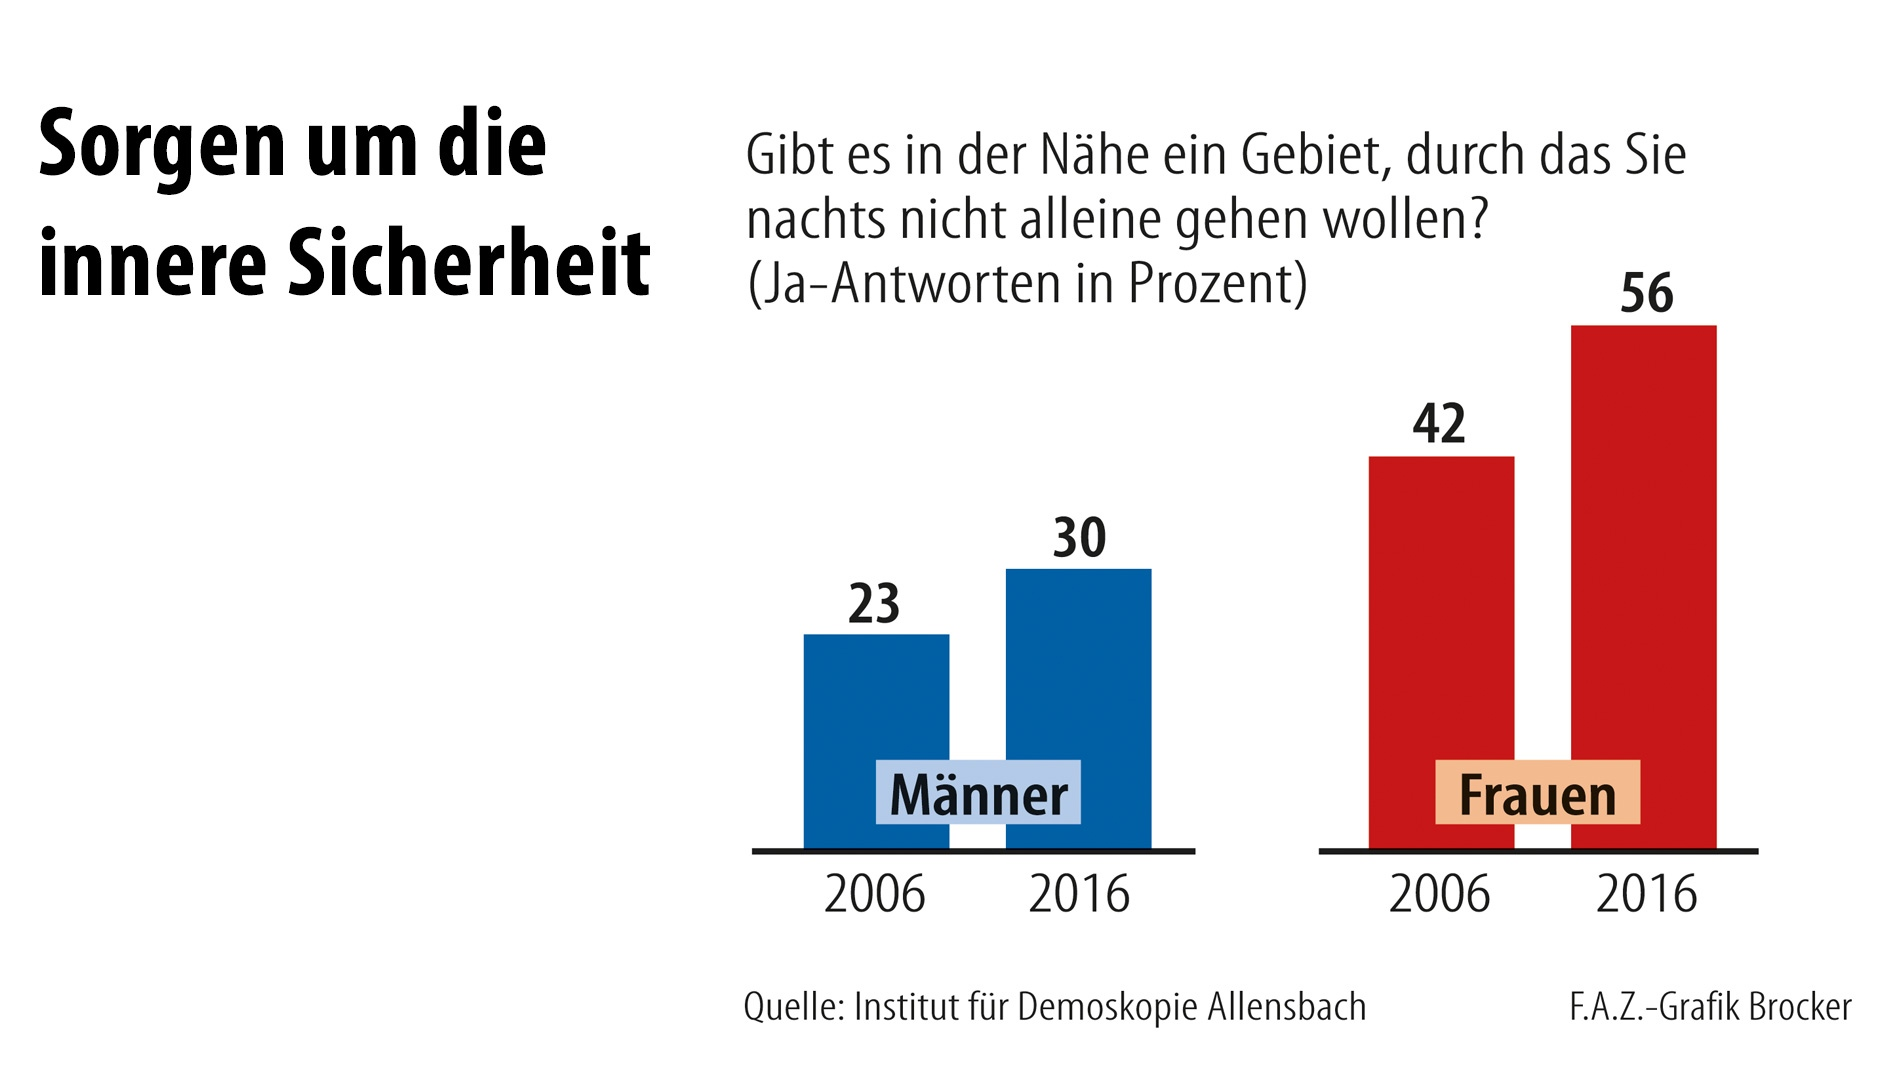
\includegraphics[width=0.85\textwidth]{sorgen.jpg}%{overlap3.pdf}
 	\end{figure}
\end{frame}

\begin{frame}{Untersuchungsdaten: Allensbach-Umfrage}
\begin{itemize}
\item{ 
Befragter Personenkreis:
Deutsche Wohnbevölkerung ab 16 Jahre in 
der Bundesrepublik Deutschland}
\item{Anzahl der Befragten:
1521
Befragungszeitraum:
01. Februar bis 11. Februar 2016}
\item{Methode:
Repräsentative Quotenauswahl
Art der Interviews:
Mündlich-persönliche Interviews}
\end{itemize}
\end{frame}

\begin{frame}{Punktschätzer für den Anteilswert}
\begin{itemize}
\item{Bei der Punktschätzung geht es darum, einen Parameter in der Grundgesamtheit
zu schätzen. Mit Bezug auf obige Grafik können wir uns z. B. für den Anteil der Männer
interessieren, die 2016 ein Gebiet in ihrer Nähe kennen, durch das Sie nachts nicht alleine gehen wollen.}
\item{Der entspreche Anteil in der Stichprobe ist $30\%.$}\pause
\item{Es ist plausibel, den in der Stichprobe beobachteten Anteilswert als Schätzer
für die Grundgesamtheit zu verwenden.}\pause
\item{Wie schätzen also, dass in Deutschland $30\%$ der deutschen ab 16 Jahren diese Frage mit 
ja beantworten. Aber wie sicher ist die Schätzung?}
\end{itemize}
% eigentlich kennen sie beides schon
% annahme es wären 100 befragte
\end{frame}
% siehe confi3.r
\begin{frame}{Ein Konfidenzintervall für den Anteilswert: Menge aller beibehaltenen Nullhypothesen}
\begin{itemize}
\item{Auf S. 52 ihrer Formelsammlung ist das Konfidenzintervall für den
Anteilswert definiert.}\pause
\item{Sie können dieses Konfidenzintervall interpretieren, als ein Intervall,
dass alle Nullhypothesen enthält, die der approximative Binomialtest beibehalten würde.}\pause
\item{Wenn man eine Stichprobe von  $100$ Männern hat, von denen $30$ die Frage bejahen, ergibt sich 
$[0.22,0.40]$ }\pause
\item{Wenn man eine Stichprobe von  $1000$ Männern hat, von denen $300$ die Frage bejahen, ergibt sich 
$[0.27,0.33]$ }
\end{itemize}
\end{frame}
% Chi-Test: Aber wie groß sind die Anteilswerte? -> Übung
% Hatten wir schon gesehen in PISA und eine Interpretation können wir schon sofort angeben

% http://www.faz.net/aktuell/politik/inland/allensbach-umfrage-zeigt-angst-um-innere-sicherheit-steigt-14073805/infografik-sorgen-um-die-14074061.html
\begin{frame}{Eine andere Interpretation des Konfidenzintervall}
\begin{itemize}
\item{Im folgenden gehen wir davon aus, dass der wahre (und unbekannte) Anteil der männlichen Personen ab
16 Jahren, die der Frage zustimmen, in der Grundgesamtheit bei $25\%$ liegt.}\pause
\item{Stellen Sie sich vor wir erheben $100$ Stichproben mit je $100$ Personen aus der Grundgesamtheit.}\pause
\item{Wir gehen dabei davon aus, dass die Grundgesamtheit so groß ist, dass keine Person doppelt vorkommt.}\pause
\item{Sie können sich vorstellen, dass $Personen$ losgehen und jede Person eine Stichprobe mit je
$100$ Personen zieht.}\pause
\item{Die Folgenden Grafiken zeigen 
\begin{itemize}
\item[1)]{das Histogramm der $100$ berechneten Anteilswerte und}
\item[2)]{die entsprechenden Konfidenzintervalle}
\end{itemize}
}
\end{itemize}
\end{frame}

\begin{frame}{Beobachtete Anteilswerte: 100 Befragungen}
%http://www.faz.net/aktuell/politik/inland/allensbach-umfrage-zeigt-angst-um-innere-sicherheit-steigt-14073805/infografik-sorgen-um-die-14074061.html
  \begin{figure}[ht]
 	\centering
 	      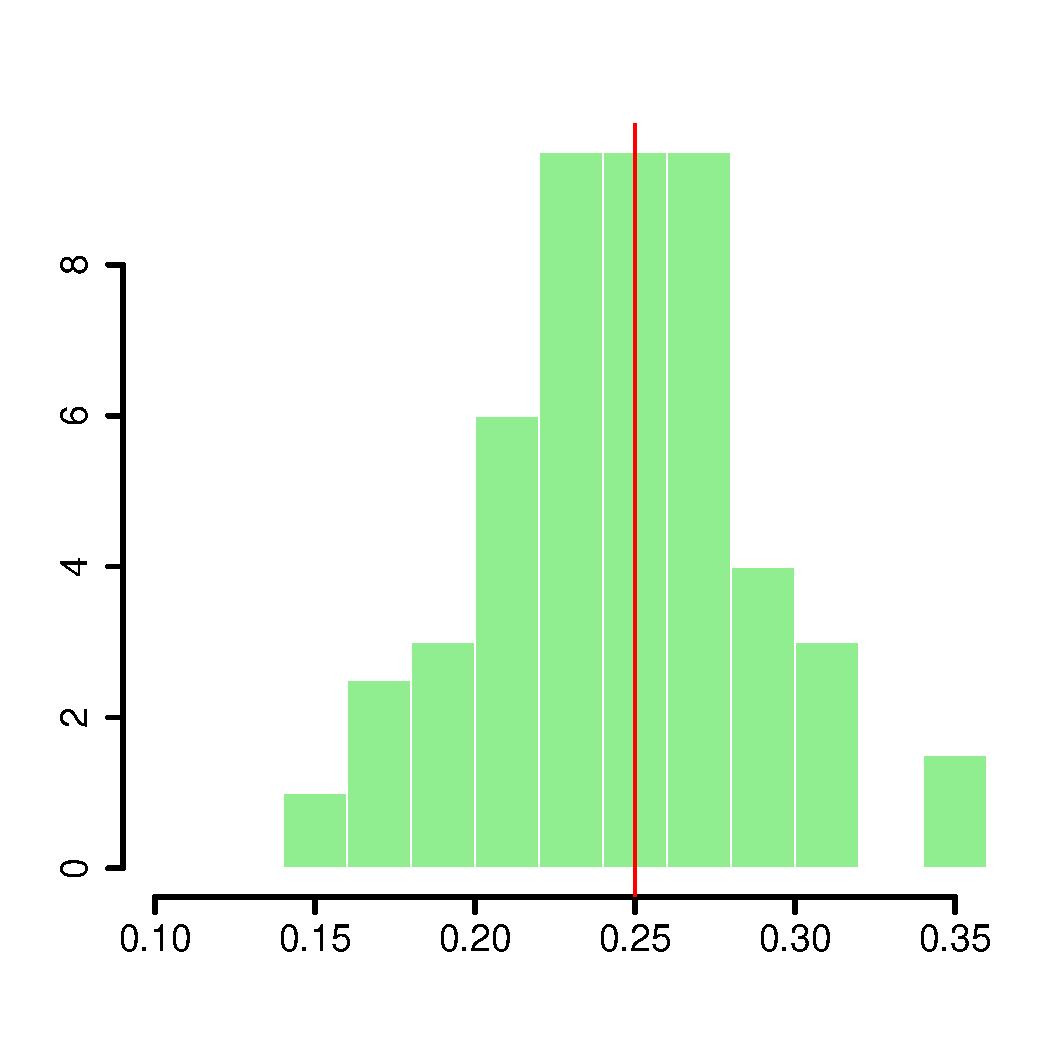
\includegraphics[width=0.65\textwidth]{prob_est.pdf}%{overlap3.pdf}
 	\end{figure}
\end{frame}

\begin{frame}{Konfidenzintervalle zu den Anteilswerten: 100 Befragungen}
%http://www.faz.net/aktuell/politik/inland/allensbach-umfrage-zeigt-angst-um-innere-sicherheit-steigt-14073805/infografik-sorgen-um-die-14074061.html
  \begin{figure}[ht]
 	\centering
 	      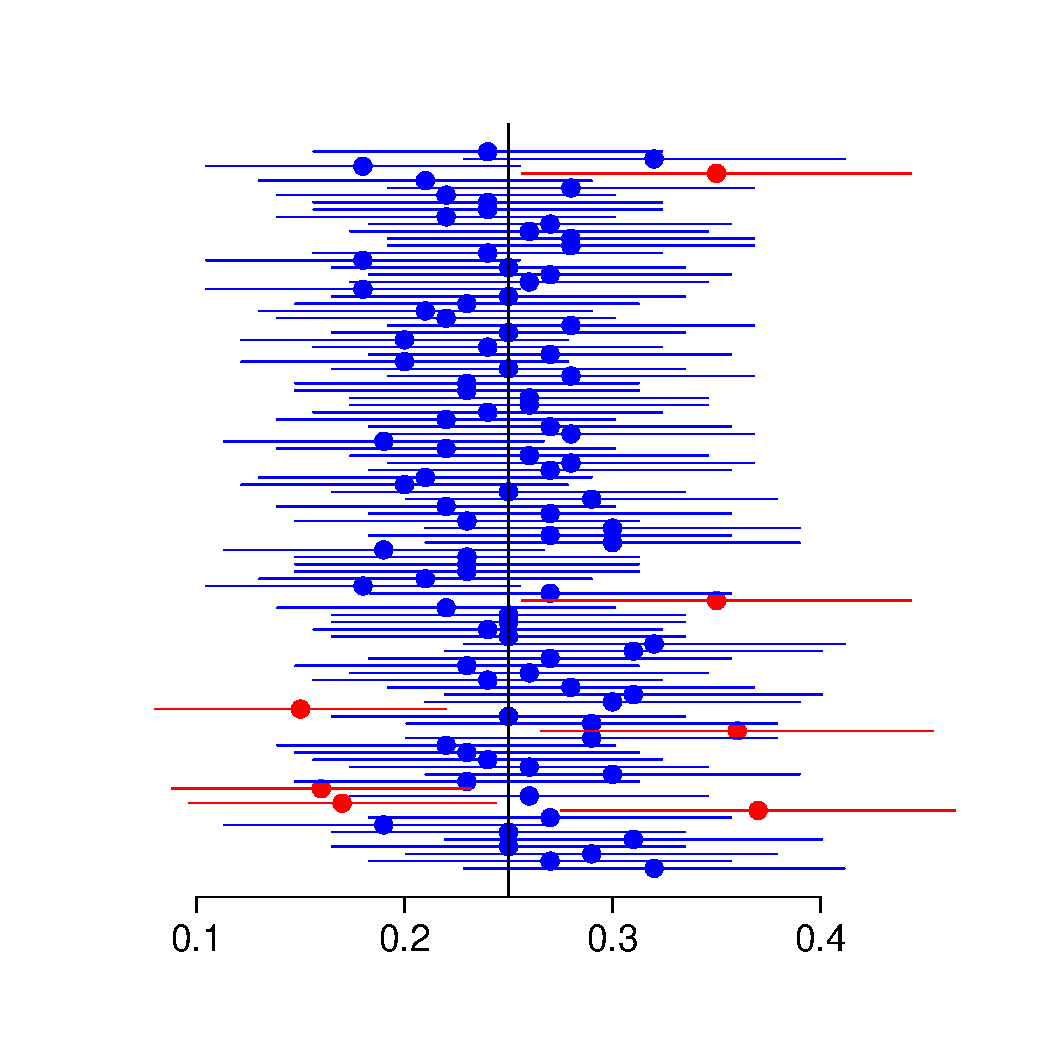
\includegraphics[width=0.65\textwidth]{confi.pdf}%{overlap3.pdf}
 	\end{figure}
\end{frame}

\begin{frame}{Betrachtung der Ergebnisse}
\begin{itemize}
\item{Von den $100$ Personen, die losgegangen sind, um jeweils eine Stichprobe von  $100$ Personen
zu ziehen, haben fünf eine Stichprobe gezogen, deren Konfidenzintervall den wahren Wert nicht
enthält.
}\pause
\item{Die anderen $95$ haben eine Stichprobe gezogen, deren Konfidenzintervall, den wahren Wert enthält.}\pause
\item{Wir wiederholen das Experiment. Diesmal gehen 500 Personen los um jeweils 100 Personen zu befragen.}\pause
\item{Was erwarten Sie? Wie viele Konfidenzintervalle werden den wahren Anteilswert nicht enthalten?}
\end{itemize}
\end{frame}

\begin{frame}{Beobachtete Anteilswerte: 200 Befragungen}
%http://www.faz.net/aktuell/politik/inland/allensbach-umfrage-zeigt-angst-um-innere-sicherheit-steigt-14073805/infografik-sorgen-um-die-14074061.html
  \begin{figure}[ht]
 	\centering
 	      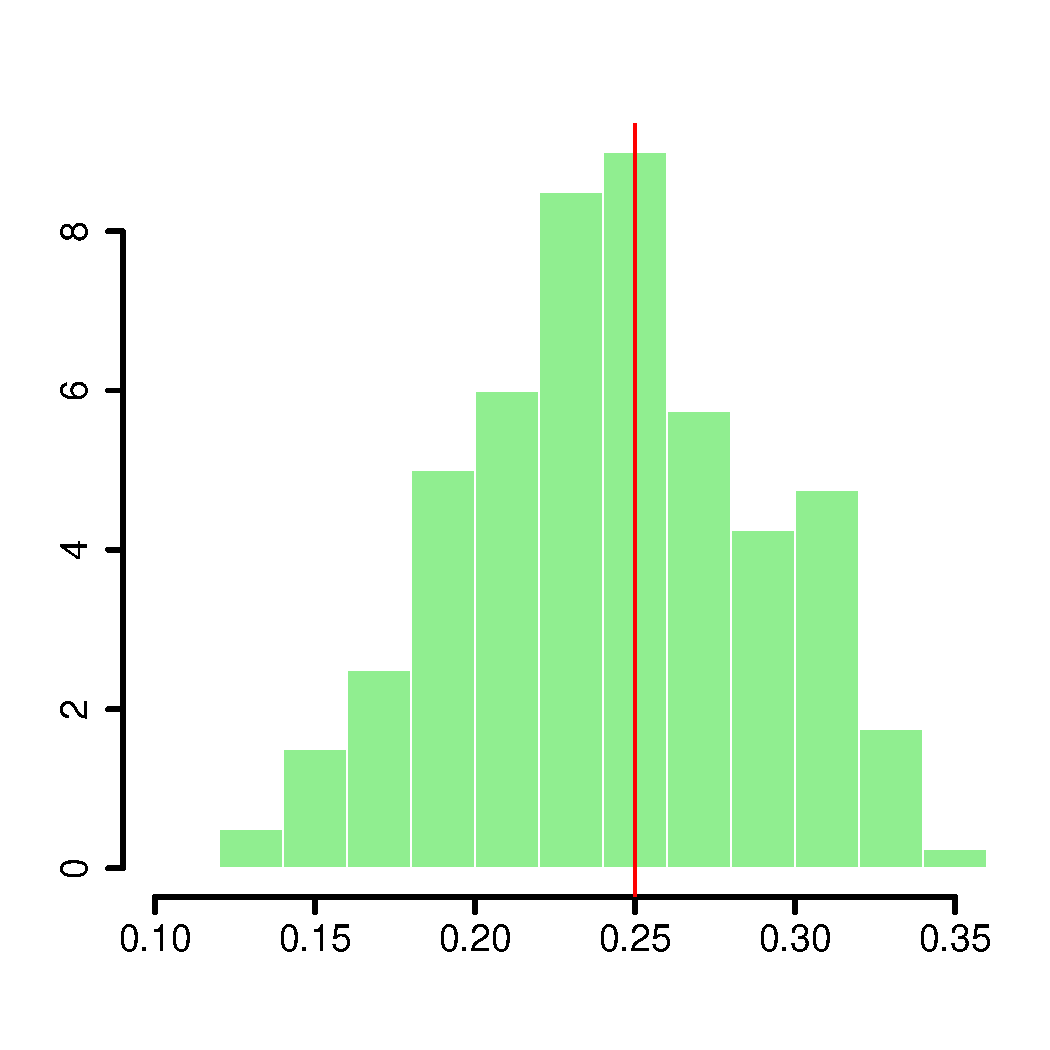
\includegraphics[width=0.65\textwidth]{prob_est200.pdf}%{overlap3.pdf}
 	\end{figure}
\end{frame}

\begin{frame}{Konfidenzintervalle zu den Anteilswerten: 200 Befragungen}
%http://www.faz.net/aktuell/politik/inland/allensbach-umfrage-zeigt-angst-um-innere-sicherheit-steigt-14073805/infografik-sorgen-um-die-14074061.html
  \begin{figure}[ht]
 	\centering
 	      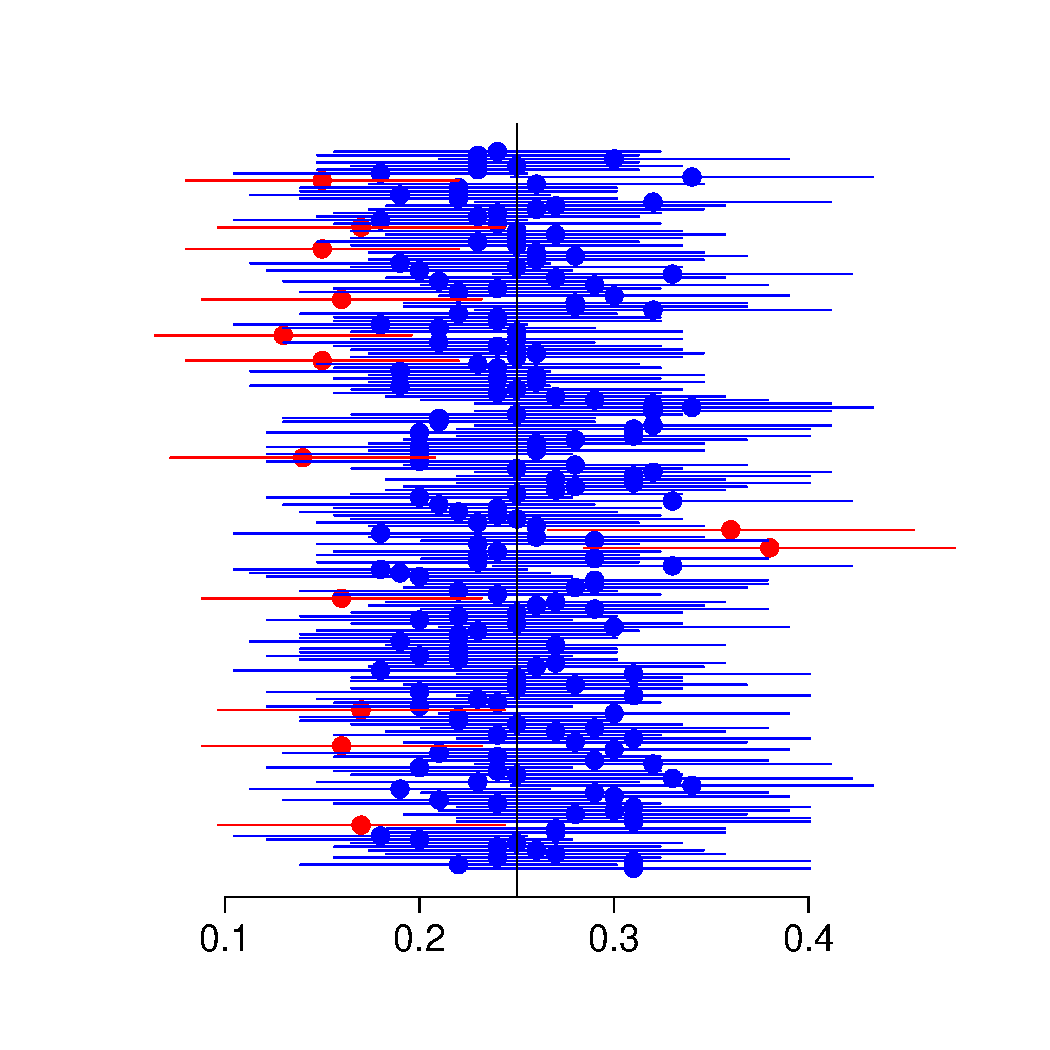
\includegraphics[width=0.65\textwidth]{confi200.pdf}%{overlap3.pdf}
 	\end{figure}
\end{frame}

\begin{frame}{Beobachtete Anteilswerte: 250 Befragungen}
%http://www.faz.net/aktuell/politik/inland/allensbach-umfrage-zeigt-angst-um-innere-sicherheit-steigt-14073805/infografik-sorgen-um-die-14074061.html
  \begin{figure}[ht]
 	\centering
 	      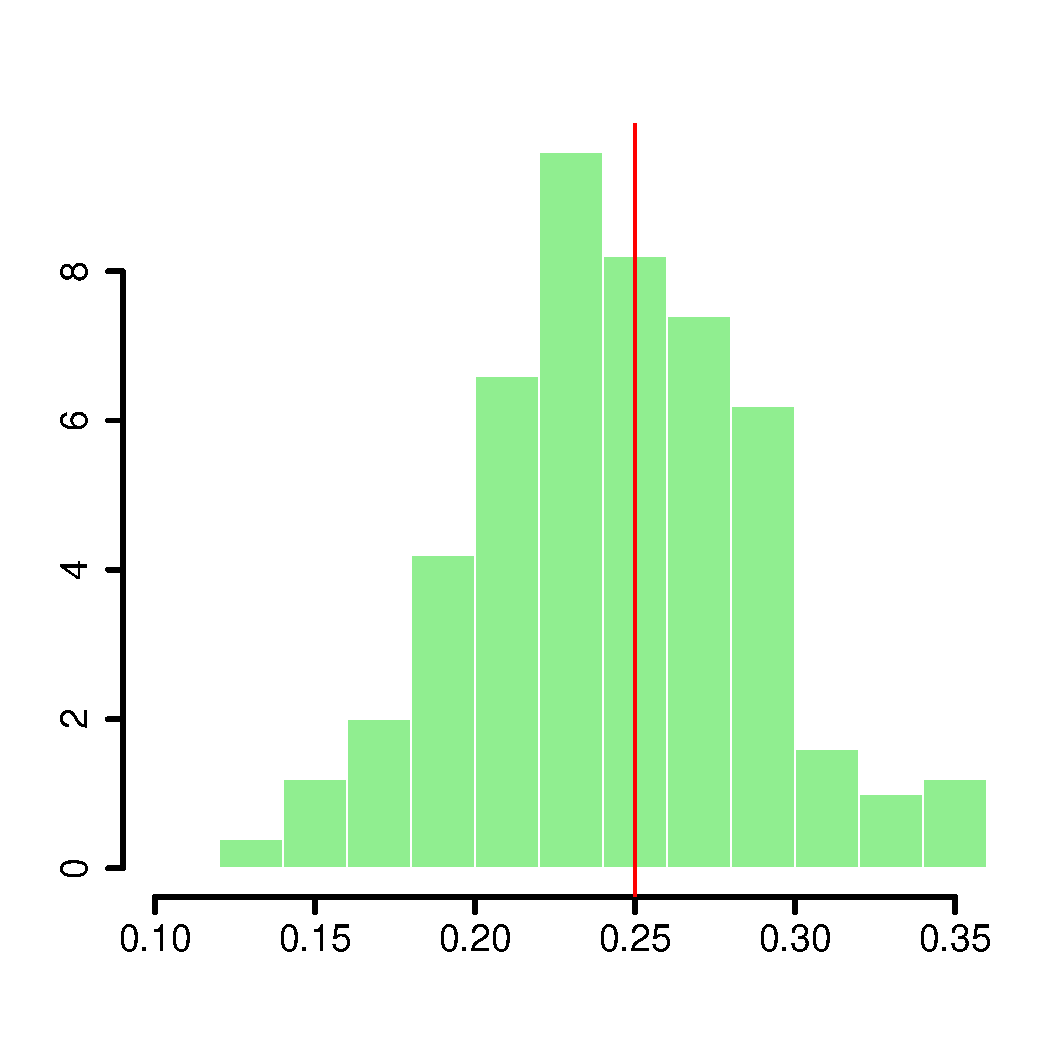
\includegraphics[width=0.65\textwidth]{prob_est250.pdf}%{overlap3.pdf}
 	\end{figure}
\end{frame}

\begin{frame}{Konfidenzintervalle zu den Anteilswerten: 250 Befragungen}
%http://www.faz.net/aktuell/politik/inland/allensbach-umfrage-zeigt-angst-um-innere-sicherheit-steigt-14073805/infografik-sorgen-um-die-14074061.html
  \begin{figure}[ht]
 	\centering
 	      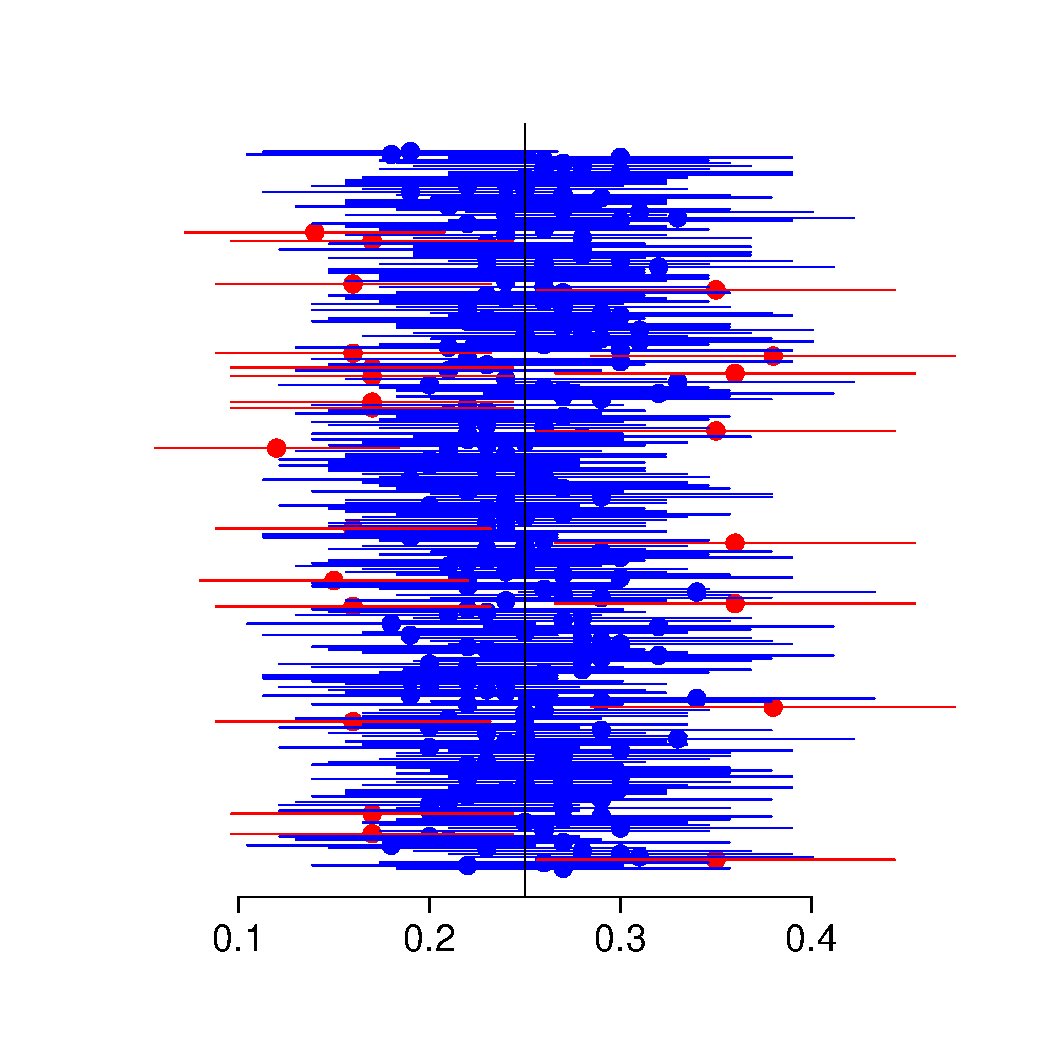
\includegraphics[width=0.65\textwidth]{confi250.pdf}%{overlap3.pdf}
 	\end{figure}
\end{frame}
% Stichprobenverteilung mit Verweise auf LMLG
% Def: Konfidenzintervall
% Zurück zum Beispiel
\begin{frame}{Allensbach-Umfrage : 100 Befragungen}
%http://www.faz.net/aktuell/politik/inland/allensbach-umfrage-zeigt-angst-um-innere-sicherheit-steigt-14073805/infografik-sorgen-um-die-14074061.html
  \begin{figure}[ht]
 	\centering
 	      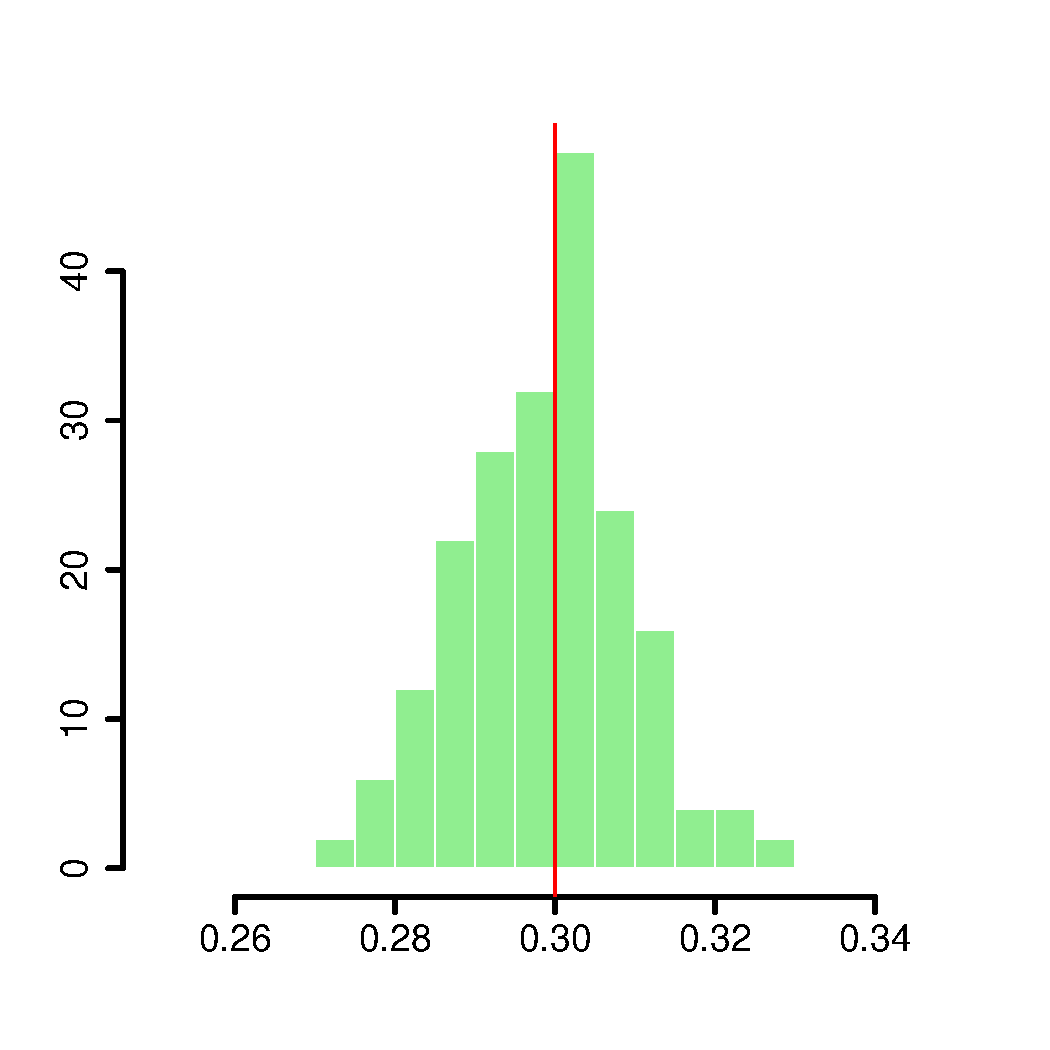
\includegraphics[width=0.65\textwidth]{umfrageEst.pdf}%{overlap3.pdf}
 	\end{figure}
\end{frame}

\begin{frame}{Allensbach-Umfrage: 100 Befragungen}
%http://www.faz.net/aktuell/politik/inland/allensbach-umfrage-zeigt-angst-um-innere-sicherheit-steigt-14073805/infografik-sorgen-um-die-14074061.html
  \begin{figure}[ht]
 	\centering
 	      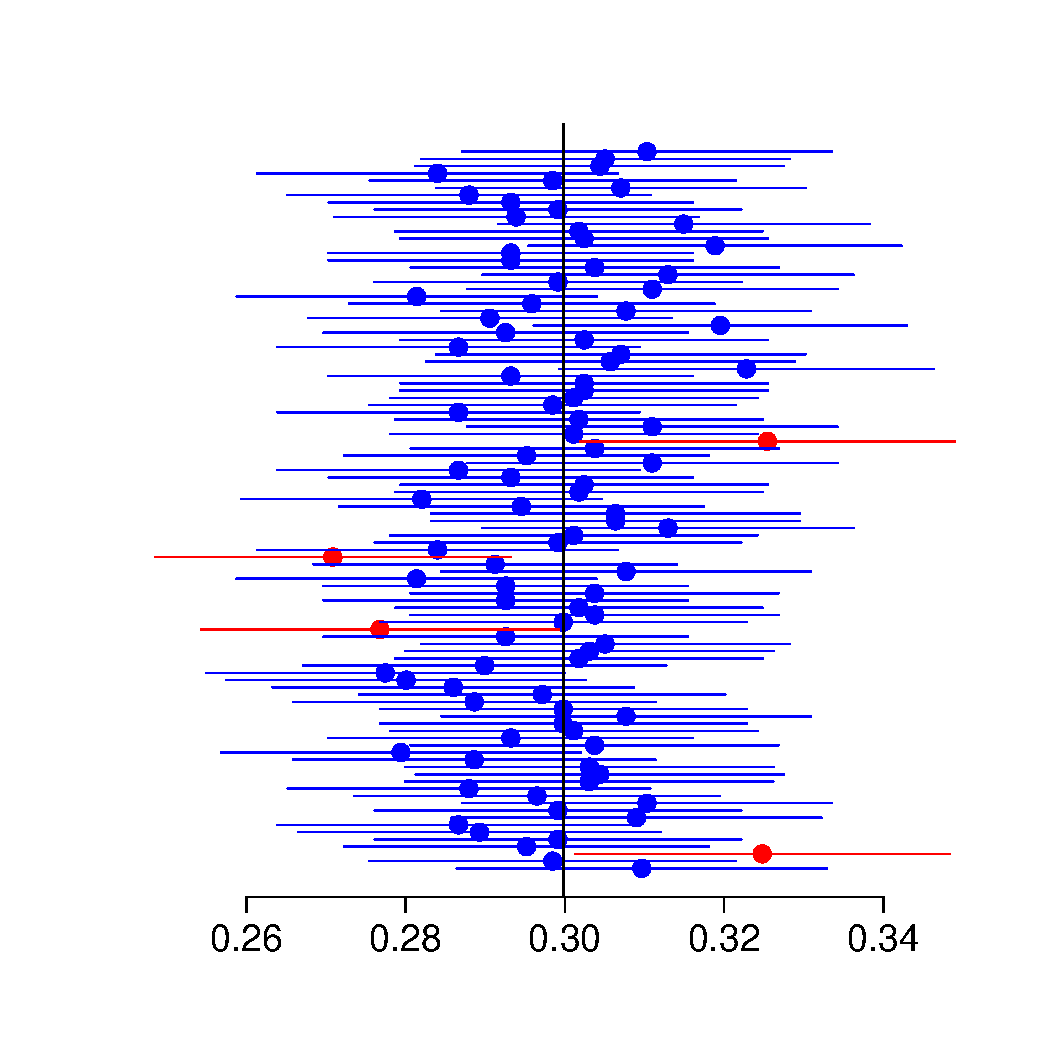
\includegraphics[width=0.65\textwidth]{umfrageConfi.pdf}%{overlap3.pdf}
 	\end{figure}
\end{frame}
% Man beachte: Es sind genau so viele falsch, aber das Intervall ist kürzer.
% Zu den paprametrischen Test gibt es auch ein entsprechendes Konfidenzintervall
\end{document}

